\chapter{Architektura aplikacji sterującej drużyną robotów \label{chap:stp}}
Przed przystąpieniem do prac nad aplikacją sterującą drużyną robotów dokonano przeglądu stosowanych rozwiązań przez uczestników mistrzostw. Okazało się, że wstępnie opracowana
architektura jest zbieżna z już istniejącym modelem nazwanym \mbox{\texttt{STP - Skill Tactics Play}} szerzej opisany w publikacji \texttt{STP: Skills, tactics and plays for multi-robot
control in adversarial environments} \cite{stp} stworzonym przez grupę naukowców z Carnegie Mellon University. Rozwiązanie to było stosowane przez drużynę \texttt{CMD Dragons} w kilku mistrzostwach.
Architektura \texttt{STP} zakłada planowanie działań drużyny na 3 poziomach:
\begin{enumerate}
 \item Poziom położony najwyżej w hierachii: \texttt{Play},
 \item \texttt{Tactics},
 \item \texttt{Skills}.
\end{enumerate}
Szczegóły algorytmu są zaprezentowane w kolejnych podrozdziałach.
\section{Opis algorytmu sterujacego drużyną}
Problem sterowania i koorydynacji działań w obrębie drużyny robotów nie jest zadaniem trywialnym. Po pierwsze środowisko w którym znajdują się roboty jest dynamiczne,
odrębym problemem jest analizowanie na bieżąco działań drużyny przeciwnej. Oczekiwania stawiane przed takim algorytmem są następujące:
\begin{itemize}
 \item koordynacja działań w obrębie drużyny mająca za zadanie osiągnięcie długofalowych celów (oddanie strzału na bramkę, a w efekcie zwycięstwo),
 \item reagowanie w czasie rzeczywistym (\textit{on-line}) na zachowania drużyny przeciwnej,
 \item budowa modelu dynamicznego świata na podstawie niepewnej informacji z czujników,
 \item modułowa architektura, umożliwiająca łątwą konfigurację i adaptację do bieżącej sytuacji.
\end{itemize}

Nazwa \texttt{STP} odnosi się bezpośrednio do modułu sztucznej inteligencji odpowiadającego za sterowanie drużyną robotów. Jak sam skrót wskazuje, podejscie 
zakłada planowanie działań na kilku poziomach. Hierarchia ma za zadanie ułatwić adaptację i paramteryzowanie poszczególnych zachowań.
Oryginalny algorytm zakłada istnienie następujących modułów:
\begin{enumerate}
  \item zawierającego informacje o świecie,
  \item umożliwiający ocenę sytuacji na planszy (pozwalający na ocenę atrakcyjności zachowań, punktów docelowych etc),
  \item sztucznej inteligencji; moduł ten powienien być odpowiedzialny za koordynację działań drużyny (tutaj właściwie realizowane jest \texttt{STP}),
  \item modułu odpowiedzialnego za nawigację robota;moduł ten powinien być odpowiedzialny za tworzenie bezkolizyjnej ścieżki prowadzącej do zadanego celu,
  \item moduł sterowania ruchem robota;
  moduł ten powinien wyznaczyć optymalne prędkości prowadzące do zadanego punktu (problem bezwładności robota,
  wyhamowanie przed punktem docelowym etc.),
  \item moduł bezpośrednio odpowiedzialny za sterowanie warstwą fizyczną robota (zadawanie prędkości liniowej kątowej, uruchamianie urządzenia do prowadzenia 
  piłki(\textit{dribbler-a}), kopnięcie piłki).
\end{enumerate}
Wszystkie warstwy algorytmu oraz przepływ informacji zostały zobrazowane na rysunku \ref{fig:stp}.
\begin{figure}[h]
\centering
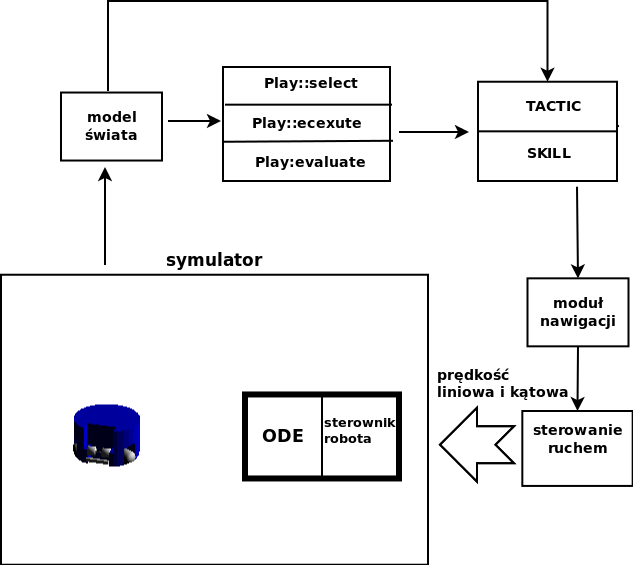
\includegraphics[scale=0.5]{./stp/stp.png}
\caption{ Architektura aplikacji sterującej drużyną.} \label{fig:stp}
\end{figure}
 \subsection*{Podstawowe pojęcia}
Właściwe planowanie działań drużyny realizowane jest na $3$ poziomach. Każdy odnosi się do innej warstwy abstrakcji.
\begin{enumerate}
  \item Poziomem najwyżej w hierachii jest \texttt{Play}. Przez to pojęcie rozumiany jest plan gry dla całej drużyny, uwzględniana jest tutaj koordynacja
  poczynań pomiędzy zawodnikami. Plan zakłada przydział roli dla każdego zawodnika. W obrębie danego planu zawodnik wykonuje swoją rolę, aż do momentu
  zakończenia danego planu lub wyznaczenia kolejnego.
  \item Przez \texttt{Tactics} rozumiany jest plan działań dla jednej roli. Można rozumieć to jako plan działań na szczeblu robota prowadzący
 do osiągnięcia pożądanego w danej sytuacji fektu. Przykładem może być strzał na bramkę. Robot dostaje polecenie oddania strzału na bramkę, zatem plan jego poczynań ma doprowadzić
 do sytuacji, w której osiągnie on pozycję umożliwiającą strzał na bramkę z zadanym powodzeniem.
 Plan na szczeblu pojedynczego robota jest wykonywany do momentu zmiany planu gry całej druzyny.
 Przykładowe plany działań dla robotów:
 \begin{itemize}
  \item strzał na bramkę,
  \item podanie piłki,
  \item odebranie podania,
  \item blokowanie innego robota,
  \item wyjście na pozycję,
  \item bronienie pozycji,
  \item dryblowanie z piłką.
 \end{itemize}

  \item Pojęcie \texttt{Skills} odnosi się do konkretnych umiejętności robota, takich jak:
    \begin{itemize}
    \item doprowadzenie piłki do celu piłki,
    \item przemieszczenie robota do celu,
    \item podążanie za innym robotem,
    \end{itemize}
  Na tym szczeblu zachowanie robota zmieniane jest w każdym kroku gry. Z każdego zadania, w każdym momencie określone musi być przejście
  albo do nowego zadania bądź kontynuowanie tego samego zadania. Przykładowo jeśli zlecimy robotowi przemieszczenie do celu z piłką i piłka 
  odskoczy robotowi, to powinien do niej podjechać i ponownie prowadzić lub jeśli nastąpi dobra okazja do strzału wykorzystać ją.
\end{enumerate}

Koordynacja poczynań drużyny zapewniona jest na najwyższym poziomie. Dodatkowo każdy poziom wprowadza dodatkowe parametry wykorzystywane przy wykonywaniu
zadania na najniższym poziomie.
Wykonywanie każdego planu \texttt{Play} wymaga spełnienia określonych predykatów, np. czy mamy rozpoczęcie gry z autu, czy wystąpił rzut rożny.

\todo{dokonczyc rozdział opisac zrealizowana wersje algorytmu}
\todo{opisać naiwny model swiata}
\todo{opisać modul oceny}
\todo{wspomniec ze rrt to modul nawigacji}